\clearpage
\section{Testable Predictions and Observational Signatures}
  \label{sec:testable-predictions-and-observational-signatures}

  Before detailing specific observational signatures, it is useful to emphasize the
  general origin of the phenomenology predicted by the Cosmochrony framework.
  The monotonic relaxation of the $\chi$ substrate, together with the topological
  organization of localized projectable configurations, generically leads to a set of
  qualitative and semi-quantitative signatures that distinguish Cosmochrony from
  standard cosmological and quantum approaches.

  It is therefore important to clarify the epistemic status of the numerical estimates
  presented in this section.
  Values such as the $\sim 8$--$10\%$ offset between early- and late-time effective
  determinations of the Hubble constant or the $\sim 10^{-10}\,\mathrm{yr}^{-1}$ drift in
  effective spacetime observables are not proposed as precision predictions.
  They should be understood as order-of-magnitude consistency estimates derived from
  the geometric coupling between the $\chi$ substrate and the effective relaxation
  fraction $\Omega_\chi$.

  Their role is to demonstrate that the Cosmochrony framework operates within a
  phenomenologically relevant regime, capable of addressing current observational
  tensions without fine-tuning or the introduction of additional dynamical degrees
  of freedom.

  \subsection{Hubble Constant from \texorpdfstring{$\chi$}{χ} Dynamics}
  \label{subsec:hubble-constant-from-chi-dynamics}

  An implication of the relaxation dynamics developed in
  Section~\ref{subsec:emergent-hubble-law} is that, in Cosmochrony,
  the Hubble parameter is not introduced as a free cosmological constant, but arises
  as an effective quantity associated with the irreversible relaxation of the
  $\chi$ substrate.

  At the level of an effective spacetime description, it may be written as
  \begin{equation}
    H(t) = \frac{\dot{\chi}}{\chi},
  \end{equation}
  where the dot denotes differentiation with respect to an effective cosmological
  time parameter introduced solely to parametrize the relaxation ordering, not a
  fundamental temporal evolution.

  In homogeneous regimes, the relaxation rate approaches its maximal admissible
  value.
  Assuming $\dot{\chi}_{\mathrm{eff}} \simeq c$, the present-day Hubble parameter can
  be estimated as
  \begin{equation}
    H_0 \simeq \frac{c}{\chi(t_0)}.
  \end{equation}

  This relation establishes a direct correspondence between the observed Hubble
  constant and the characteristic relaxation scale of $\chi$ at the current epoch.
  Early-universe probes (such as CMB-based inferences) and late-time distance-ladder
  measurements effectively sample $\chi$ at different stages of its relaxation,
  naturally leading to systematically different inferred values of $H_0$ without
  invoking additional cosmological components or fine-tuned initial conditions.

  \paragraph{Resolution of the Hubble tension.}
    The modulation of the $\chi$ relaxation rate by large-scale matter
    inhomogeneities provides a natural mechanism for reconciling early-universe and
    late-time measurements of the Hubble constant.
    Within this framework, the effective Hubble parameter $H(z)$ acquires a mild
    redshift dependence that departs from the $\Lambda$CDM expectation at intermediate
    redshifts ($0.1 \lesssim z \lesssim 10$).
    This deviation reflects the partial projectability of the relaxation dynamics in
    inhomogeneous regimes, rather than the presence of additional cosmological
    components.
    The resulting behavior is directly testable through upcoming baryon acoustic
    oscillation and supernova surveys.

% Requires: \usepackage{pgfplots}
% Optional: \pgfplotsset{compat=1.18}
    \begin{figure}[t]
      \centering
      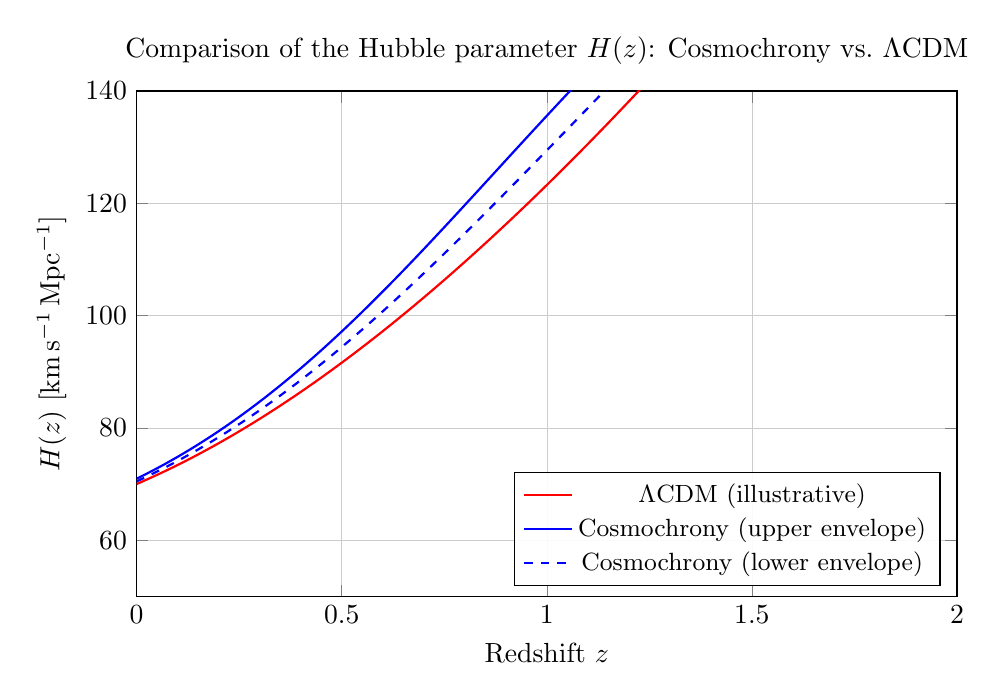
\begin{tikzpicture}
        \begin{axis}[
          width=12cm,
          height=8cm,
          title={Comparison of the Hubble parameter $H(z)$: Cosmochrony vs.\ $\Lambda$CDM},
        xlabel={Redshift $z$},
        ylabel={$H(z)$ [km\,s$^{-1}$\,Mpc$^{-1}$]},
        xmin=0, xmax=2,
        ymin=50, ymax=140,
        xtick={0,0.5,1,1.5,2},
        legend style={
          at={(rel axis cs:0.98,0.02)},
          anchor=south east,
          draw=black,
          fill=white,
          fill opacity=0.9,
          text opacity=1,
          font=\small
        },
        grid=both,
        grid style={line width=.1pt, draw=gray!10},
        major grid style={line width=.2pt, draw=gray!40},
        ]

          % --- Baseline LCDM ---
          \addplot[
            domain=0:2, samples=200,
            red, thick, mark=none
          ]
          {70*sqrt(0.3*(1+x)^3 + 0.7)};
          \addlegendentry{$\Lambda$CDM (illustrative)}

          % --- Cosmochrony band ---
          \addplot[
            domain=0:2, samples=200,
            blue, thick, mark=none
          ]
          {70*sqrt(0.3*(1+x)^3 + 0.7) * (1 + 0.10*exp(-2*(x-1)^2))};
          \addlegendentry{Cosmochrony (upper envelope)}

          \addplot[
            domain=0:2, samples=200,
            blue, thick, dashed, mark=none
          ]
          {70*sqrt(0.3*(1+x)^3 + 0.7) * (1 + 0.05*exp(-2*(x-1)^2))};
          \addlegendentry{Cosmochrony (lower envelope)}
        \end{axis}
      \end{tikzpicture}
      \caption{Schematic comparison of $H(z)$ in Cosmochrony and $\Lambda$CDM.
      Cosmochrony predicts a mild enhancement at intermediate redshifts due to
      relaxation inhomogeneities, providing a discriminating observational test.}
      \label{fig:hubble-comparison}
    \end{figure}

  \subsection{Redshift Drift}
  \label{subsec:redshift-drift}

  An implication of the monotonic relaxation dynamics developed in
  Section~\ref{subsec:expansion-as-relaxation} is that cosmological
  redshifts exhibit a slow temporal evolution when described in an effective
  spacetime parametrization.
  This leads to a redshift drift whose magnitude and redshift dependence differ
  quantitatively from those predicted by the standard $\Lambda$CDM model,
  particularly at intermediate redshifts.

  At the level of an effective parametrization, intended only as an order-of-magnitude
  estimate rather than a derived dynamical law, the effective drift rate may be
  written as
  \begin{equation}
    \dot{z}_{\mathrm{eff}}
    \;\sim\;
    H_0 (1+z) - \frac{c}{\chi(t)},
  \end{equation}
  where the second term reflects the ongoing relaxation of the $\chi$ substrate rather
  than a dark-energy-driven acceleration.
  This corresponds to a secular variation of order
  \[
    \Delta z \sim 10^{-10}\,\mathrm{yr}^{-1}
  \]
  at redshift $z \sim 1$, differing from $\Lambda$CDM expectations at the
  $\sim 10\%$ level in this regime.

  Future high-precision spectroscopic facilities, such as extremely large telescopes
  equipped with ultra-stable spectrographs, may be capable of probing this effect.
  A detection of a redshift drift incompatible with $\Lambda$CDM predictions would
  therefore provide a direct observational discriminator between geometric
  relaxation of the $\chi$ substrate and dark-energy-driven cosmic acceleration.

  \subsection{Gravitational Wave Propagation}
  \label{subsec:gravitational-wave-propagation}

  In the Cosmochrony framework, gravitational waves correspond to propagating
  collective modulations of the $\chi$ field in regimes where a spacetime
  description is applicable.
  They do not constitute independent propagating degrees of freedom, but reflect
  time-dependent redistributions of relaxation constraints within the field.

  In regions of high excitation density, such as near compact objects, the local
  slowdown of $\chi$ relaxation is expected to modify the propagation of these
  modulations.
  In particular, partial decoherence or attenuation may arise due to the coupling
  of propagating modulations to strongly constrained relaxation regions.
  These effects originate from the same collective relaxation constraints
  responsible for gravitational time dilation and horizon formation, and do not
  require the introduction of additional dynamical fields.

  \paragraph{Order-of-magnitude attenuation estimate.}
    Consider a compact object of mass $M$, characterized in effective geometric
    descriptions by a Schwarzschild radius
    \[
      r_s = \frac{2GM}{c^2}.
    \]
    Gravitational-wave modulations of the $\chi$ field propagating through regions
    where the effective relaxation rate is significantly reduced are expected to lose
    coherence through partial redistribution into non-propagating relaxation modes.

    For waves traversing regions within a characteristic distance
    \[
      r \lesssim 10\,\frac{GM}{c^2},
    \]
    the cumulative reduction of effective relaxation conductivity suggests an
    attenuation factor that may be parametrized, at the level of order-of-magnitude
    estimates, as
    \[
      \frac{\Delta A}{A} \sim \mathcal{O}(10^{-2} - 10^{-1}),
    \]
    where the precise magnitude depends on the local $\chi$ correlation length $\xi$
    and on the effective relaxation fraction $\Omega_\chi$ in the vicinity of the
    source.
    This attenuation should be interpreted as a redistribution of wave coherence
    within the $\chi$ relaxation dynamics rather than as dissipative energy loss in
    the conventional field-theoretic sense.

  \paragraph{Observational signature.}
    Such effects are expected to manifest most clearly during the late-time ringdown
    phase of binary black hole mergers, where gravitational-wave signals probe the
    strongly constrained relaxation regime near the effective horizon.
    The resulting signature would appear as a frequency-dependent deviation from
    general relativistic ringdown templates, potentially mimicking anomalous damping
    or mode-dependent quality factors.

    While current ground-based detectors do not yet achieve the signal-to-noise ratios
    required to resolve attenuation at the few-percent level, future space-based
    observatories operating in the LISA band, with expected signal-to-noise ratios
    exceeding $\sim 100$ for massive black hole mergers, may provide sufficient
    sensitivity to test this prediction.

  \paragraph{Semi-quantitative scaling estimate.}
    Within the Cosmochrony framework, attenuation of gravitational-wave amplitudes
    near compact objects arises from the local suppression of $\chi$ relaxation in
    regions of high effective curvature.
    At leading order, the relative amplitude reduction is expected to scale with the
    dimensionless curvature parameter $(r_s / r)$.

    A simple dimensional estimate yields
    \[
      \frac{\Delta A}{A} \sim \left( \frac{r_s}{r} \right)^2 ,
    \]
    indicating that the effect depends explicitly on both the compact object mass and
    the wave trajectory’s impact parameter.
    For propagation at distances $r \approx 10\,r_s$, this scaling gives
    \[
      \frac{\Delta A}{A} \sim 10^{-2},
    \]
    consistent with the order-of-magnitude estimates above and with exploratory
    numerical results obtained from $\chi$-field simulations
    (Appendix~D.3).

  \subsection{Galaxy Rotation Curves from Structural Relaxation}
  \label{subsec:galaxy-rotation-chi}

  As shown in Section~\ref{subsec:phi-eff-galaxies}, the Cosmochrony framework
  predicts modifications of galactic rotation curves arising from the structural
  relaxation of the projected \(\chi_{\mathrm{eff}}\) field, without introducing
  additional dark matter components.

  The Cosmochrony framework predicts modifications of galactic rotation curves arising
  from the structural relaxation of the projected \(\chi_{\mathrm{eff}}\) field, without
  introducing additional dark matter components.

  In regions where localized matter configurations induce persistent relaxation
  gradients in the \(\chi\)-substrate, the effective inertial response of orbiting matter
  is modified.
  This leads to an enhancement of tangential velocities at large radii, producing
  approximately flat rotation curves.

  Unlike modified gravity scenarios, this effect does not require an explicit change of
  the gravitational force law.
  It arises from a non-local redistribution of relaxation capacity in the projected
  description, tied to the large-scale coherence of the underlying \(\chi\)-configuration.

  Observable consequences include:
  \begin{itemize}
    \item a correlation between rotation curve flattening and indicators of structural
    relaxation activity rather than baryonic mass alone,
    \item deviations from simple baryonic scaling relations in dynamically young or
    disturbed galaxies,
    \item a reduced need for fine-tuned dark matter profiles in low-surface-brightness
    systems.
  \end{itemize}

  These signatures provide a discriminant between Cosmochrony, particle dark matter
  models, and purely phenomenological modified gravity approaches.

  \subsection{Spin and Topological Signatures}
  \label{subsec:spin-and-topological-signatures}

  An implication of the topological origin of spin developed in
  Section~\ref{subsec:spin_topology} is that, if particle spin originates from
  topologically nontrivial configurations of the $\chi$ substrate, then spin-related
  phenomena may admit geometric signatures not captured by purely algebraic quantum
  descriptions.

  In particular, ultra-high-precision interference experiments sensitive to
  $4\pi$ rotational symmetry may, in principle, probe deviations associated with
  the internal topology of localized projectable $\chi$ configurations.
  Such deviations would not modify standard spin--statistics relations, but could
  appear as extremely small phase shifts or coherence effects under closed
  $2\pi$ versus $4\pi$ rotational cycles.

  These signatures are expected to be strongly suppressed and therefore lie beyond
  current experimental resolution.
  However, their existence would provide a conceptually distinctive test of the
  topological origin of spin proposed in Cosmochrony, as opposed to interpretations
  in which spin is treated as an abstract representation of spacetime symmetry
  groups.

  \input{14-predictions/06-absence-of-dark-energy-signatures}
  \subsection{CMB Polarization Signatures (Outlook)}
  \label{subsec:cmb-polarization-signatures}

  As discussed in Section~\ref{subsec:cmb}, residual large-scale projective correlations
  inherited from the pre-geometric relaxation of the $\chi$ substrate are expected to
  imprint scale-dependent signatures on the Cosmic Microwave Background (CMB).
  In Cosmochrony, these correlations arise from the bounded and irreversible relaxation
  of $\chi$, locally constrained by the invariant speed $c$, without invoking any
  superluminal stretching or inflationary phase.
  As a consequence, correlations at the largest angular scales are naturally suppressed,
  leading to a reduction of power at low multipoles ($\ell \lesssim 10$).
  This mechanism is consistent with several large-angle features reported in CMB data,
  such as hemispherical asymmetry, without requiring fine-tuned initial conditions.
  Quantitative estimates of the resulting low-$\ell$ attenuation are discussed in
  Appendix~\ref{app:lowell_attenuation}.

  Observationally, the \emph{Planck} 2018 data report a suppression of the CMB quadrupole
  power at the level of $\sim 10\%$ relative to the $\Lambda$CDM best-fit expectation,
  corresponding to the long-standing low-$\ell$ anomaly at $\ell = 2$~\cite{Aghanim2020}.
  Within Cosmochrony, this suppression arises naturally from the pre-geometric relaxation
  dynamics of the $\chi$ substrate, which reduces large-angle correlations prior to the
  emergence of an effective spacetime description.
  Unlike phenomenological explanations relying on specific initial conditions or
  model-dependent modifications of primordial spectra, the effect follows directly from
  the intrinsic relaxation properties of the underlying field.

  \paragraph{Cosmological Imprints: The \texorpdfstring{$8/3$}{8/3} Scaling in CMB Polarization}
    \label{subsec:cmb_8_3_scaling}

    Beyond temperature anisotropies, the fundamental spectral ratio
    $\lambda_2/\lambda_1 = 8/3$, which governs the electroweak mass hierarchy at the
    micro-scale (see Appendix~\ref{sec:spectral_ratio_derivation}), is expected to leave a
    structural signature in the polarization sector of the CMB.
    In this framework, primordial scalar and tensor perturbations are reinterpreted as
    dual manifestations of the substrate's relaxation, corresponding respectively to
    base transmittance and fiber shear modes of the projection.

    \subparagraph{Geometric Bound on the Tensor-to-Scalar Ratio (\texorpdfstring{$r$}{r})}

      In Cosmochrony, the tensor-to-scalar ratio $r$ is constrained by the relative spectral
      stiffness of the $\chi$ substrate's projection modes.
      Under the principle of \textbf{Projective Spectral Saturation} at the high-energy limit
      ($k \approx 1/h_\chi$), the relaxation energy $\mathcal{E}$ is distributed according to
      the maximal kinematic capacity of each mode:
    \begin{equation}
      \mathcal{E}_s \propto \lambda_{\text{base}} \Delta_s^2,
      \qquad
      \mathcal{E}_t \propto \lambda_{\text{fiber}} \Delta_t^2 .
      \end{equation}
      The ``bare'' geometric ratio $r_0$ is defined by the saturation of these spectral densities:
    \begin{equation}
      r_0
      = \frac{\Delta_t^2}{\Delta_s^2}
      = \frac{\lambda_{\text{base}}}{\lambda_{\text{fiber}}}
      = \frac{3}{8}
      \simeq 0.375 .
      \end{equation}
      This value does not correspond to an observable tensor-to-scalar ratio at recombination,
      but defines a \emph{geometric upper bound} imposed by the topology of the projection fiber
      at the saturation scale.

    \subparagraph{Topological Decoherence and Parametrization of \texorpdfstring{$r_{\text{obs}}$}{robs}}

      The observed ratio $r_{\text{obs}}$ undergoes \textbf{topological decoherence} as the
      substrate expands.
      Since fiber shear modes are intrinsically more sensitive to losses of projective
      alignment, the cumulative degradation of alignment induces a monotonic suppression
      of tensor modes.
      To leading order, this effect may be effectively parametrized as
    \begin{equation}
      r_{\text{obs}}(t)
      = r_0 \cdot \exp\!\left( -\zeta \frac{\tau_\chi}{t} \right),
      \end{equation}
      where $\tau_\chi$ denotes the characteristic relaxation time of the substrate.
      The precise functional form is not fundamental and merely encodes the fact that fiber
      shear modes decohere faster than base transmittance during cosmic relaxation.
      This decay represents the transition from the primordial saturated state to the
      present large-scale geometric stability, providing a structural explanation for the
      low observed value of $r$ ($r < 0.036$), without invoking slow-roll dynamics or
      fine-tuned inflationary potentials.

  \subsection{Neutrino-Mediated Relaxation and Decay Signatures}
  \label{subsec:neutrino-decay-signatures}

  An implication of the structural interpretation of particle decay
  (Section~\ref{subsec:metastability-and-decay}) together with
  the partial projectability of neutrino modes
  (Section~\ref{subsec:neutrinos-partially-projectable-modes}) is that, in
  Cosmochrony, particle decay and neutrino emission are manifestations of structural
  reorganization rather than independent microscopic processes.
  This interpretation leads to distinct observational signatures.

  Because neutrino-like excitations act as non-local relaxation channels, decay processes
  in the early universe contribute to an irreversible smoothing of admissible configurations.
  This smoothing is expected to leave detectable imprints across multiple observational domains.

  Specifically, the framework predicts:
  \begin{itemize}
    \item an enhanced role of neutrino backgrounds in suppressing large-scale coherence
    without behaving as conventional radiation pressure,
    \item a weak coupling between decay rates and late-time environmental conditions,
    reflecting their origin in early structural metastability,
    \item possible correlations between decay-driven neutrino emission and large-scale
    anisotropies observed in the cosmic microwave background.
  \end{itemize}

  At the particle-physics level, this interpretation suggests that decay lifetimes and
  branching ratios encode information about the stability landscape of admissible
  projected configurations rather than fundamental stochasticity.
  Future precision measurements of rare decays may therefore provide indirect probes of
  the structural relaxation dynamics underlying the Cosmochrony framework.

  \subsubsection*{Environmental Modulation of Particle Stability}
    \label{subsec:environmental-decay-modulation}

    A distinctive prediction of the Cosmochrony framework is that particle stability is not
    strictly universal, but may exhibit a weak dependence on the surrounding structural environment.
    Because particle decay originates from the susceptibility of metastable projected
    configurations to their own admissible fluctuations, any factor that modifies the local
    relaxation landscape can, in principle, affect decay rates.

    In regions characterized by strong gradients of the \(\chi\) substrate—such as galactic
    cores or highly structured gravitational environments—the spectrum and amplitude of
    admissible fluctuations are expected to differ slightly from those in weakly structured
    regions.
    As a result, the effective lifetime of unstable particles may acquire a small environment-dependent modulation.

    This effect is predicted to be extremely weak and therefore compatible with all current
    laboratory and astrophysical constraints.
    Nevertheless, it represents a qualitatively new signature: a violation of strict
    universality of decay rates induced not by local interactions or spacetime curvature,
    but by structural relaxation gradients in the underlying relational substrate.

    Future high-precision measurements of decay processes in environments with strong
    gravitational or structural gradients, as well as dedicated numerical simulations of
    \(\chi\)-field dynamics, may allow quantitative estimates of this effect.
    Its detection or exclusion would provide a direct and stringent test of the Cosmochrony framework.

    \paragraph{Order-of-magnitude estimate.}

      Within the Cosmochrony framework, the effective lifetime of an unstable particle is
      controlled by the susceptibility of a metastable projected configuration to its own
      admissible fluctuations.
      Because the spectrum and density of such fluctuations depend weakly on the surrounding
      structural environment, a small modulation of decay rates is expected in regions
      characterized by strong gradients of the \(\chi\) substrate.

      A minimal parametrization of this effect may be written as
    \begin{equation}
      \frac{\delta \Gamma}{\Gamma}
      \;\simeq\;
      \beta\,\frac{\Delta U}{c^2},
      \end{equation}
      where \(\Gamma\) is the decay rate, \(U\) denotes an effective gravitational or
      structural potential serving as a proxy for the local relaxation gradient, and
      \(\beta\) is a dimensionless sensitivity coefficient encoding the response of the
      projected configuration to environmental variations.

      Existing tests of local position invariance based on high-precision atomic clocks
      strongly constrain any environmental dependence of effective physical rates.
      Requiring compatibility with these constraints suggests a conservative bound
      \(\beta \lesssim 10^{-6}\).

      For typical galactic environments, the difference in effective potential between
      weakly structured regions and galactic cores is of order
      \(\Delta U / c^2 \sim 10^{-7}\)–\(10^{-6}\).
      Combining these estimates yields a fractional modulation of particle lifetimes of
      order
    \begin{equation}
      \frac{\delta \tau}{\tau}
      \;\sim\;
      10^{-13}\text{--}10^{-12}.
      \end{equation}

      Such an effect is far below the sensitivity of current laboratory measurements and
      therefore fully compatible with existing experimental bounds.
      Nevertheless, it represents a qualitatively novel signature: a weak violation of the
      strict universality of decay rates induced not by spacetime curvature or local
      interactions, but by structural relaxation gradients in the underlying relational
      substrate.
      Future high-precision astrophysical observations or dedicated numerical simulations of
      \(\chi\)-field dynamics may allow this prediction to be further quantified or
      constrained.

    \paragraph{Which decay channels are most sensitive?}

      In Cosmochrony, an environmental modulation of decay rates is expected to be largest
      for metastable configurations whose admissible fluctuation spectrum is only weakly
      protected by topology, and whose decay proceeds through a comparatively ``thin''
      projective channel (small number of admissible final factorizable branches).
      This suggests the following qualitative hierarchy of experimental leverage:

    \begin{itemize}
      \item \textbf{Purely leptonic weak decays} (e.g.\ \(\mu^\pm \to e^\pm \nu \bar{\nu}\)):
      theoretically clean (minimal hadronic uncertainty), with extremely well-characterized
      kinematics. The limitation is practical: \(\tau_\mu\) is measured very precisely, but
      changing the \emph{structural environment} sufficiently in the laboratory is difficult.

      \item \textbf{Hadronic weak decays and oscillating neutral mesons}
      (e.g.\ \(K^0\)--\(\bar{K}^0\), \(B^0\)--\(\bar{B}^0\)):
      in standard physics these are exquisitely sensitive to tiny perturbations in the
      effective Hamiltonian. In Cosmochrony terms, they probe whether the projection fiber
      admits a detectable environment-dependent bias between conjugate branches.
      The price is interpretability: hadronic and medium effects require careful control.

      \item \textbf{Nuclear \(\beta\)-decays and long-lived isotopes}:
      exceptionally good metrological stability allows long integration times, but nuclear
      structure systematics are harder to disentangle from any putative projective effect.

      \end{itemize}

      Overall, the cleanest conceptual target is leptonic weak decay, while the most
      ``amplified'' interferometric target is neutral-meson mixing, provided that standard
      environmental systematics are tightly controlled.

    \paragraph{Differential astrophysical signature.}

      Directly comparing lifetimes of unstable particles between ``void'' and typical
      galactic cores is observationally challenging, because decay processes are not
      tagged \emph{in situ}.
      However, Cosmochrony predicts a \emph{differential} effect that can in principle be
      searched for in environments where the effective potential proxy \(\Delta U/c^2\)
      is substantially larger than in ordinary galactic regions.

      In particular, energetic hadronic cascades near compact objects (accretion flows and
      relativistic jets) are controlled by the competition between interaction lengths and
      decay lengths of \(\pi^\pm\), \(K^\pm\), and \(\mu^\pm\), which shapes the emergent
      high-energy \(\gamma\)-ray and neutrino spectra.
      If decay rates acquire a weak environmental modulation,
    \begin{equation}
      \frac{\delta \Gamma}{\Gamma} \simeq \beta\,\frac{\Delta U}{c^2},
      \end{equation}
      then the \emph{effective} critical energy at which decay dominates over interaction
      is shifted by the same fractional amount,
    \begin{equation}
      \frac{\delta E_\ast}{E_\ast} \sim \frac{\delta \tau}{\tau}
      \sim \beta\,\frac{\Delta U}{c^2}.
      \end{equation}

      Near the innermost regions of accretion flows around massive compact objects,
      a characteristic scale \(\Delta U/c^2 \sim 10^{-4}\) is not excluded as an order-of-magnitude proxy,
      leading (for conservative \(\beta \lesssim 10^{-6}\)) to
    \begin{equation}
      \frac{\delta \tau}{\tau} \sim 10^{-10},
      \end{equation}
      still extremely small, but conceptually clean: a systematic, environment-correlated
      spectral bias that cannot be mimicked by late-time cosmological parameter shifts.

      The key discriminant is \emph{correlation with environment}:
      sources with otherwise similar intrinsic properties but different compactness proxies
      (e.g.\ inferred emission radius or gravitational redshift indicators) should exhibit
      a tiny but coherent shift in the decay-limited spectral features of hadronic secondaries.

    \paragraph{Connection to numerical \(\chi\)-field simulations.}

      The sensitivity coefficient \(\beta\) can be operationally defined and extracted from
      \(\chi\)-field simulations by measuring how the \emph{escape time} of a metastable
      localized configuration changes when embedded in a controlled background gradient.

      Let \(\tau_0\) denote the mean first-passage (escape) time of a metastable localized
      configuration in a reference background, estimated from an ensemble of runs with
      different admissible fluctuation seeds.
      Introduce a dimensionless structural gradient proxy \(G\) (computed from the projected
      field) such as
    \begin{equation}
      G \;\equiv\; \frac{\ell^2}{\chi_0^2}\,\langle |\nabla \chi_{\mathrm{eff}}|^2 \rangle_{\mathcal{R}},
      \end{equation}
      where \(\ell\) is a chosen coarse-graining scale, \(\chi_0\) a normalization, and
      \(\langle \cdot \rangle_{\mathcal{R}}\) denotes averaging over a region \(\mathcal{R}\)
      containing the localized excitation.

      Define the empirical susceptibility
    \begin{equation}
      S \;\equiv\; \frac{d\ln \tau}{dG},
      \end{equation}
      estimated numerically by repeating the experiment at slightly different controlled
      background gradients \(G\).
      A minimal mapping to the phenomenological parametrization
      \(\delta\tau/\tau \simeq \beta\,\Delta U/c^2\) is then obtained by specifying an
      effective correspondence between \(\Delta U/c^2\) and \(\Delta G\) in the simulation,
    \begin{equation}
      \frac{\delta \tau}{\tau} \;\simeq\; S\,\Delta G
      \;\equiv\; \beta\,\frac{\Delta U}{c^2}.
      \end{equation}

      In practice, this provides a clear numerical pipeline:
      (i) prepare a metastable localized configuration, (ii) embed it in backgrounds with
      controlled \(G\), (iii) estimate \(\tau(G)\) from ensembles, and (iv) infer \(S\),
      hence \(\beta\), up to the chosen environment proxy mapping.
      The resulting \(\beta\) can then be confronted with the conservative metrological
      requirement \(\beta \lesssim 10^{-6}\).

  \subsection{Environmental Modulation of Particle Lifetimes}
  \label{subsec:environmental-modulation-lifetimes}

  Within the Cosmochrony framework, particle decay is not interpreted as a
  fundamental stochastic process, but as the manifestation of the
  \emph{structural susceptibility} of a metastable projected configuration
  to admissible fluctuations of the underlying relational substrate $\chi$.
  As discussed in Section~\ref{subsec:neutrino-decay-signatures}, these
  fluctuations form a bounded background whose spectral density depends
  weakly on the local relaxation structure of $\chi$.

  As a consequence, the decay rate $\Gamma$ of an unstable particle is not
  strictly universal, but may exhibit an extremely small environmental
  dependence reflecting variations in the local relaxation gradient of the substrate.
  At leading order, this effect may be parametrized as
  \begin{equation}
    \frac{\delta \Gamma}{\Gamma}
    \;\simeq\;
    \beta \, \frac{\Delta U}{c^{2}},
    \label{eq:lifetime-modulation}
  \end{equation}
  where $U$ denotes an effective gravitational or structural potential
  serving as a proxy for the local relaxation density, and $\beta$ is a
  dimensionless sensitivity parameter encoding the coupling between the
  projected metastable configuration and the admissible substrate fluctuations.

  Since the particle lifetime is given by $\tau = \Gamma^{-1}$, the relative
  variation of the lifetime satisfies, to first order,
  \begin{equation}
    \frac{\delta \tau}{\tau}
    \;\simeq\;
    - \frac{\delta \Gamma}{\Gamma}.
  \end{equation}

  Existing experimental constraints on local position invariance, in
  particular those derived from high-precision atomic clock comparisons,
  suggest a conservative upper bound $\beta \lesssim 10^{-6}$.
  Typical contrasts in effective potential between weakly structured
  environments and regions of high structural density (e.g.\ galactic
  cores) correspond to $\Delta U / c^{2} \sim 10^{-7}$--$10^{-6}$.
  Under these conditions, Cosmochrony predicts
  \begin{equation}
    \frac{\delta \tau}{\tau}
    \;\sim\;
    10^{-13} \text{--} 10^{-12},
    \label{eq:lifetime-order-of-magnitude}
  \end{equation}
  well below current laboratory sensitivities, but conceptually distinct
  from standard quantum or relativistic effects.

  Importantly, this modulation does not arise from spacetime curvature,
  local interactions, or environmental decoherence, but from the structural
  properties of the non-injective projection from $\chi$ to its effective
  description.
  A future detection of even a minute, reproducible deviation from strict lifetime universality would therefore
  constitute a direct signature of the underlying relational substrate.

  \subsection{Summary}
  \label{subsec:summary6}

  Within the Cosmochrony framework, gravity does not arise as a fundamental interaction
  or as an independent geometric degree of freedom.
  It emerges at the level of effective descriptions as a macroscopic consequence of
  localized projected configurations collectively constraining admissible relaxation
  ordering.

  Classical gravitational phenomena—including gravitational time dilation, effective
  spacetime curvature, gravitational waves, and black holes—are recovered as distinct
  descriptive regimes of this collective constraint.
  They reflect variations in the projectability and correlation structure of admissible
  descriptions, rather than the dynamics of a fundamental spacetime or gravitational
  field.

  In this perspective, gravitation appears as an emergent, operational phenomenon,
  summarizing how localized projected configurations collectively limit admissible
  ordering and correlation across extended regions, without introducing gravity as a
  primitive force or fundamental geometric entity.

